% Options for packages loaded elsewhere
\PassOptionsToPackage{unicode}{hyperref}
\PassOptionsToPackage{hyphens}{url}
\PassOptionsToPackage{dvipsnames,svgnames,x11names}{xcolor}
%
\documentclass[
  letterpaper,
  DIV=11,
  numbers=noendperiod]{scrartcl}

\usepackage{amsmath,amssymb}
\usepackage{iftex}
\ifPDFTeX
  \usepackage[T1]{fontenc}
  \usepackage[utf8]{inputenc}
  \usepackage{textcomp} % provide euro and other symbols
\else % if luatex or xetex
  \usepackage{unicode-math}
  \defaultfontfeatures{Scale=MatchLowercase}
  \defaultfontfeatures[\rmfamily]{Ligatures=TeX,Scale=1}
\fi
\usepackage{lmodern}
\ifPDFTeX\else  
    % xetex/luatex font selection
\fi
% Use upquote if available, for straight quotes in verbatim environments
\IfFileExists{upquote.sty}{\usepackage{upquote}}{}
\IfFileExists{microtype.sty}{% use microtype if available
  \usepackage[]{microtype}
  \UseMicrotypeSet[protrusion]{basicmath} % disable protrusion for tt fonts
}{}
\makeatletter
\@ifundefined{KOMAClassName}{% if non-KOMA class
  \IfFileExists{parskip.sty}{%
    \usepackage{parskip}
  }{% else
    \setlength{\parindent}{0pt}
    \setlength{\parskip}{6pt plus 2pt minus 1pt}}
}{% if KOMA class
  \KOMAoptions{parskip=half}}
\makeatother
\usepackage{xcolor}
\setlength{\emergencystretch}{3em} % prevent overfull lines
\setcounter{secnumdepth}{5}
% Make \paragraph and \subparagraph free-standing
\ifx\paragraph\undefined\else
  \let\oldparagraph\paragraph
  \renewcommand{\paragraph}[1]{\oldparagraph{#1}\mbox{}}
\fi
\ifx\subparagraph\undefined\else
  \let\oldsubparagraph\subparagraph
  \renewcommand{\subparagraph}[1]{\oldsubparagraph{#1}\mbox{}}
\fi


\providecommand{\tightlist}{%
  \setlength{\itemsep}{0pt}\setlength{\parskip}{0pt}}\usepackage{longtable,booktabs,array}
\usepackage{calc} % for calculating minipage widths
% Correct order of tables after \paragraph or \subparagraph
\usepackage{etoolbox}
\makeatletter
\patchcmd\longtable{\par}{\if@noskipsec\mbox{}\fi\par}{}{}
\makeatother
% Allow footnotes in longtable head/foot
\IfFileExists{footnotehyper.sty}{\usepackage{footnotehyper}}{\usepackage{footnote}}
\makesavenoteenv{longtable}
\usepackage{graphicx}
\makeatletter
\def\maxwidth{\ifdim\Gin@nat@width>\linewidth\linewidth\else\Gin@nat@width\fi}
\def\maxheight{\ifdim\Gin@nat@height>\textheight\textheight\else\Gin@nat@height\fi}
\makeatother
% Scale images if necessary, so that they will not overflow the page
% margins by default, and it is still possible to overwrite the defaults
% using explicit options in \includegraphics[width, height, ...]{}
\setkeys{Gin}{width=\maxwidth,height=\maxheight,keepaspectratio}
% Set default figure placement to htbp
\makeatletter
\def\fps@figure{htbp}
\makeatother
% definitions for citeproc citations
\NewDocumentCommand\citeproctext{}{}
\NewDocumentCommand\citeproc{mm}{%
  \begingroup\def\citeproctext{#2}\cite{#1}\endgroup}
\makeatletter
 % allow citations to break across lines
 \let\@cite@ofmt\@firstofone
 % avoid brackets around text for \cite:
 \def\@biblabel#1{}
 \def\@cite#1#2{{#1\if@tempswa , #2\fi}}
\makeatother
\newlength{\cslhangindent}
\setlength{\cslhangindent}{1.5em}
\newlength{\csllabelwidth}
\setlength{\csllabelwidth}{3em}
\newenvironment{CSLReferences}[2] % #1 hanging-indent, #2 entry-spacing
 {\begin{list}{}{%
  \setlength{\itemindent}{0pt}
  \setlength{\leftmargin}{0pt}
  \setlength{\parsep}{0pt}
  % turn on hanging indent if param 1 is 1
  \ifodd #1
   \setlength{\leftmargin}{\cslhangindent}
   \setlength{\itemindent}{-1\cslhangindent}
  \fi
  % set entry spacing
  \setlength{\itemsep}{#2\baselineskip}}}
 {\end{list}}
\usepackage{calc}
\newcommand{\CSLBlock}[1]{\hfill\break\parbox[t]{\linewidth}{\strut\ignorespaces#1\strut}}
\newcommand{\CSLLeftMargin}[1]{\parbox[t]{\csllabelwidth}{\strut#1\strut}}
\newcommand{\CSLRightInline}[1]{\parbox[t]{\linewidth - \csllabelwidth}{\strut#1\strut}}
\newcommand{\CSLIndent}[1]{\hspace{\cslhangindent}#1}

\usepackage{booktabs}
\usepackage{longtable}
\usepackage{array}
\usepackage{multirow}
\usepackage{wrapfig}
\usepackage{float}
\usepackage{colortbl}
\usepackage{pdflscape}
\usepackage{tabu}
\usepackage{threeparttable}
\usepackage{threeparttablex}
\usepackage[normalem]{ulem}
\usepackage{makecell}
\usepackage{xcolor}
\usepackage{siunitx}

  \newcolumntype{d}{S[
    input-open-uncertainty=,
    input-close-uncertainty=,
    parse-numbers = false,
    table-align-text-pre=false,
    table-align-text-post=false
  ]}
  
\KOMAoption{captions}{tableheading}
\makeatletter
\@ifpackageloaded{caption}{}{\usepackage{caption}}
\AtBeginDocument{%
\ifdefined\contentsname
  \renewcommand*\contentsname{Table of contents}
\else
  \newcommand\contentsname{Table of contents}
\fi
\ifdefined\listfigurename
  \renewcommand*\listfigurename{List of Figures}
\else
  \newcommand\listfigurename{List of Figures}
\fi
\ifdefined\listtablename
  \renewcommand*\listtablename{List of Tables}
\else
  \newcommand\listtablename{List of Tables}
\fi
\ifdefined\figurename
  \renewcommand*\figurename{Figure}
\else
  \newcommand\figurename{Figure}
\fi
\ifdefined\tablename
  \renewcommand*\tablename{Table}
\else
  \newcommand\tablename{Table}
\fi
}
\@ifpackageloaded{float}{}{\usepackage{float}}
\floatstyle{ruled}
\@ifundefined{c@chapter}{\newfloat{codelisting}{h}{lop}}{\newfloat{codelisting}{h}{lop}[chapter]}
\floatname{codelisting}{Listing}
\newcommand*\listoflistings{\listof{codelisting}{List of Listings}}
\makeatother
\makeatletter
\makeatother
\makeatletter
\@ifpackageloaded{caption}{}{\usepackage{caption}}
\@ifpackageloaded{subcaption}{}{\usepackage{subcaption}}
\makeatother
\ifLuaTeX
  \usepackage{selnolig}  % disable illegal ligatures
\fi
\usepackage{bookmark}

\IfFileExists{xurl.sty}{\usepackage{xurl}}{} % add URL line breaks if available
\urlstyle{same} % disable monospaced font for URLs
\hypersetup{
  pdftitle={(No) Privacy Please!: How China Obtains Citizen Consent for Online Monitoring},
  pdfauthor={Andrew MacDonald},
  pdfkeywords={Digital Privacy, Covid-19, Authoriatrian
Regimes, Government Trust, China},
  colorlinks=true,
  linkcolor={blue},
  filecolor={Maroon},
  citecolor={Blue},
  urlcolor={Blue},
  pdfcreator={LaTeX via pandoc}}

\title{(No) Privacy Please!: How China Obtains Citizen Consent for
Online Monitoring}
\author{Andrew MacDonald}
\date{2024-09-05}

\begin{document}
\maketitle

\section{Introduction}\label{sec-introduction}

\section{Literature review}\label{sec-litreview}

\subsection{Background}\label{background}

How online users feel about government tracking of their data is a
subject that has been studied in a wide variety of contexts yet the
research has produced highly divergent results, depending on the
technology studied, the cultural context, and the exact framing of the
research question. Compounding this problem, to date, most of the
research on the topic has been conducted primarily on U.S. or Western
respondents, with comparatively fewer researchers reporting on
developing or non-democratic countries. This research agenda has taken
on new urgency during the Covid-19 pandemic, as governments around the
globe engaged in highly intrusive monitoring and data collection
activities.

From the pre-Covid privacy literature, three important findings stand
out. The first is that demographic variables are important predictors of
attitudes toward online privacy. In an important early study of early
Internet users, Sheehan has found that education and age are two
important determinants of online privacy attitudes Sheehan (2002).
Others have replicated this result and found that characteristics such
as gender, social setting, and income also play a role in forming
privacy expectations (Anwar et al., 2017; Büchi et al., 2021; Lee et
al., 2019). The second finding is that respondent personal experience
with privacy and technology is also an important factor. Malandrino et
al.~finds that users who work in ICT fields are actually less concerned
with their online privacy Malandrino et al. (2013). Dupree et
al.~suggest that there are possibly several types of online user
typologies, with user experience being a variable that matters but can
potentially shift respondents to an extreme view in either direction
Dupree et al. (2016). Gerber et al., as part of a meta-analysis of
privacy, notes that young people may be more conscious of their online
privacy context and therefore are more active in policing their privacy
boundaries Gerber and Green (2012). These findings all suggest that
personal characteristics and background are important determinants of
privacy attitudes.

The third finding, more specific to the focus of this paper, is that
trust in the state is an important predictor variable in whether
respondents feel anxious about government monitoring of their online
behavior. Pavone and Esposti found that users either trusted the
government and therefore did not find proposed monitoring concerning, or
did not trust the government and therefore believed any monitoring to be
threatening Pavone and Esposti (2012). Trüdinger and Steckermeier find
that acceptance of government surveillance in Germany depends on how
much respondents trust the state Trüdinger and Steckermeier (2017).

The literature on government monitoring of citizens increased
dramatically after the onset of the Covid-19 pandemic, though most of
the findings echo those of Pavone and Esposti and other earlier
scholars. Because the Covid-19 pandemic resulted in a wide range of new
tracking technologies, scholars have focused directly on how users and
respondents felt regarding government monitoring (for a sampling of the
vast literature, see (Abramova et al., 2022; Garrett et al., 2021;
Ioannou and Tussyadiah, 2021; Ong and Loo, n.d.; Wnuk et al., 2020)). To
highlight one example of this Covid-era research, Ioannou and Tussyadiah
highlights the linkage between state trust, surveillance acceptance, and
perceived necessity in explaining the variation in willingness to use
contact tracing apps in the U.S.

How these findings translate to the Chinese context is somewhat less
clear. While recent research has begun to develop a picture of Chinese
attitudes toward government monitoring, there are still some important
unanswered questions. Several studies have found that Chinese
respondents are generally more willing to use or accept government
surveillance technologies across several different technology types
(Habich-Sobiegalla and Kostka, 2023; Kostka et al., 2021; Kostka and
Habich-Sobiegalla, 2024). Steinhardt et al.~find that users in China
tend to trust the government with their data more than they do with
private corporations Steinhardt et al. (2022). Liu and Kostka, in
separate papers, both find that trust in the state is correlated with
increased acceptance of the social credit system (Liu) and surveillance
more broadly (Kostka) (Kostka, 2023; Liu, 2022).

\subsection{Contribution}\label{contribution}

This work aims to make two contributions to the literature on government
surveillance. First, it seeks to help clarify which demographic and
attitudinal factors are important in predicting privacy concerns.
Previous findings of support for respondent attributes that predict
acceptance of government surveillance do not find support here may
suggest features of the Chinese context that lead to this variation in
results. This variation may also apply to other non-democratic or
non-Western countries.

Second, there have been very few studies of privacy atttitudes that are
not purely cross-sectional. The survey used in this paper was conducted
in two waves, before the strict Covid controls were enacted in China,
and another wave conducted just after the controls were relaxed. During
this time, as You et al.~have found, the Chinese response to the
pandemic engendered significant criticism and resulted in a decline in
trust of government You et al. (2024). This study can help understand if
these events, and the intense government monitoring that was used to
control the pandemic, lead to any significant changes in the
relationship between state trust and acceptance of government
surveillance.

\subsection{Hypotheses}\label{hypotheses}

The existing literature and the specific features of this survey
generates a set of testable hypotheses, including:

\(H_1\): Demographic variables such as education and income predict
acceptance of government monitoring

A finding here that certain demographic factors are or are not relevant
in China may suggest some contextual factors that create differences
from China to the other areas studied.

\(H_{2a}\) Technical know-how and privacy consciousness predicts
acceptance of government monitoring

\(H_{2b}\): Technical know-how and privacy consciousness does not
predict acceptance of government monitoring

The Chinese online information environment is highly controlled,
particularly with respect to any information critical of the government.
Privacy knowledge and technical skill may therefore be uncorrelated or
positively correlated with support for government monitoring, contra the
existing literature that has been developed in the West.

\(H_3\): Trust in government should predict acceptance of government
monitoring

Both existing studies of Chinese users and those outside of China have
all found this relationship to be a relatively robust one.

\(H_4\): The pandemic experience has altered the relationship between
institutional trust and acceptance of tracking

Given the apparent decline in institutional trust as a result of the
pandemic, and the expectation derived from \(H_3\), this research
expects to find some change in the relationship between these variables.

\(H_5\): Factors that drive concern regarding government tracking should
differ from concerns regarding private tracking

This hypothesis is a somewhat speculative one, but, given that previous
research has found significant differences in the level of acceptance of
tracking between public and private sources in China, and, that trust in
government is likely not a factor for accepting private tracking, there
may be some differences in the factors that predict these two variables.

\section{Data and summary statistics}\label{sec-datasummary}

The data for this project was collected via a commercial survey firm in
two waves, February of 2021 and March of 2023. The 2021 survey had an
n=1500 and the second had an n=2000. Questions on the two surveys were
identical other than a minor change to a question that referenced a
specific date. The timing of the two surveys came at two very different
points in time of China's Covid-19 experience. The first survey was
conducted approximately seven months after the last round of
restrictions were lifted on the city of Wuhan. China, at the time, was
essentially closed to foreign travel but otherwise had little in the way
of day to day public health restrictions. Nationwide, daily Covid cases
hovered around the single digits (\emph{BBC News}, 2021). China was at a
very different point in its journey in March of 2023. The year of 2022
saw widespread, intrusive digital monitoring introduced. Many major
cities, such as Shanghai, Xi'an, and Shenzhen, underwent long and
painful city-wide lockdown procedures. At the end of 2023, under the
weight of a spiraling number of cases and widespread protests (termed
the White Paper Revolution), China finally abandoned its zero Covid
policy (Mao, 2022). The two waves of these surveys aim to compare
attitudes before and after this widespread and highly visible change in
digital monitoring strategies.

The demographics of the 2021 and 2023 surveys are presented in
Table~\ref{tbl-demographics}.

\begin{longtable}[t]{llrr}

\caption{\label{tbl-demographics}Select key demographic variables}

\tabularnewline

\toprule
  &    & Mean & Std. Dev.\\
\midrule
Age &  & 33.2 & 11.6\\
\midrule
 &  & N & Pct.\\
Location & Countryside/village & 477 & 13.6\\
 & Small city & 1059 & 30.2\\
 & Mid-sized city & 840 & 24.0\\
 & Big city & 1131 & 32.2\\
Education & No formal education & 22 & 0.6\\
 & Primary & 134 & 3.8\\
 & Middle school & 384 & 10.9\\
 & High school & 843 & 24.0\\
 & University & 1914 & 54.6\\
 & Advanced studies/Graduate school & 210 & 6.0\\
Gender & Female & 1711 & 48.8\\
 & Male & 1796 & 51.2\\
Marriage status & Single & 1101 & 31.4\\
 & In a relationship & 569 & 16.2\\
 & Married & 1744 & 49.7\\
 & Divorced & 93 & 2.7\\
Party member status & Yes & 483 & 13.8\\
 & No & 3024 & 86.2\\
Communist Youth League status & Yes & 1116 & 31.8\\
 & No & 2391 & 68.2\\
Income & 0-2,999 & 275 & 7.8\\
 & 3,000-5,999 & 822 & 23.4\\
 & 6,000-9,999 & 899 & 25.6\\
 & 10,000-19,999 & 962 & 27.4\\
 & 20,000-49,999 & 385 & 11.0\\
 & 50,000-99,999 & 94 & 2.7\\
 & More than 100,000 & 70 & 2.0\\
Year & 2021 & 1500 & 42.8\\
 & 2023 & 2007 & 57.2\\
\bottomrule

\end{longtable}

As is typical of online surveys in China, the sample respondents skew
somewhat younger and more educated. Comparing the two waves, there are
some modest demographic differences (notably education and marriage)
differences between the two samples. As will be shown in
Section~\ref{sec-analysis}, these minor differences do not appear to
change any of the substantive results. Focusing on the 2023 survey, the
modal respondent is someone from a small city, male, married, working in
a white collar job at a small enterprise, who earns about 10,000 RMB a
month and has an urban \emph{hukou}.

To simplify the analysis that follows, the variables are recoded such
that income is divided into three categories (low, middle, and high) and
education is divided into two categories, those with college education
and those without. The regressions in the following sections were tested
with alternate specifications of these categorical variables (code for
these regressions available at the author's website) and the key results
were unaffected.

\begin{table}

\caption{\label{tbl-respvarindex}Questions asking about attitudes toward
government monitoring}

\centering{

\centering
\begin{tabular}[t]{l|>{\raggedright\arraybackslash}p{5in}}
\hline
GM1 & There are good reasons for the central government to monitor the activity of users online\\
\hline
\cellcolor{gray!6}{GM2} & \cellcolor{gray!6}{There are good reasons for the local government to monitor the activity of users online}\\
\hline
TRACK1 & How comfortable are you with the central government knowing personal details about your activity online?\\
\hline
\cellcolor{gray!6}{TRACK2} & \cellcolor{gray!6}{How comfortable are you with the local government knowing personal details about your activity online?}\\
\hline
\end{tabular}

}

\end{table}%

The key response variable for the following analysis is an index
variable created by combining the results of the four questions in
Table~\ref{tbl-respvarindex}, rescaled to be between zero and one. It is
true that previous research has found that Chinese respondents place
lower levels of trust in local governments as compared to central
governments (Chen, 2017; Zhong, 2014). However, the correlation between
\texttt{GM1} and \texttt{GM2} is 0.84 and the correlation between
\texttt{TRACK1} and \texttt{TRACK2} is 0.87. Additionally, as shown in
the online appendices, each of the major regression results in
Section~\ref{sec-analysis} do not demonstrate major changes if the same
variables are regressed on each of the survey question items
individually. Indicating their close relationship, the variables taken
together have a Cronbach's \(\alpha\) of 0.81. Intuitively, this high
level of relatedness makes sense as while respondents have some
background attitudes about the difference between central and local
governments, they may not easily be able to identify at which level
government tracking occurs.

Finally, there has been some debate as to the extent of preference
falsification on online surveys in China. To test for preference
falsification, the surveys also contained several list experiment
questions. List experiments have been used in a number of surveys to
allow residents a confidential method to express their true attitudes
about topics such as racial views, sexual assault experience, and
political views (Moseson et al., 2017; Redlawsk et al., 2010). While
Glynn (Glynn (2013)) points out that list experiments should not be seen
as silver bullet to the problem of preference falsification, the results
of the list experiments (also available in the online appendices)
roughly match the answers to the component questions that comprise the
response variable index.

Overall, the survey data should provide a robust test to arbitrate
between the hypotheses posed in Section~\ref{sec-litreview}.

\section{Analysis}\label{sec-analysis}

\subsection{Predicting citizen attitudes about government
monitoring}\label{predicting-citizen-attitudes-about-government-monitoring}

The first set of models considers the question of which demographic
variables predict variation in attitudes toward being tracked by the
government. Overall, the central finding is that the demographic
variables are relatively weak predictors of acceptance of government
monitoring. The key predictor variables included in
Table~\ref{tbl-citizenatt} are the standard suite of demographic
variables, the tech savvy index (TSI), and the knowledge index (KI). The
items used to construct the two indicies variables are listed in
Section~\ref{sec-appendix}. The Cronbach's \(\alpha\) for each of the
two variables are 0.8 and 0.55 respectively, indicating that the
questions are suitable for use in an index.

\begin{table}

\caption{\label{tbl-citizenatt}Demographic predictors of attitude toward
government privacy}

\centering{

\centering
\begin{tabular}[t]{lcccccc}
\toprule
  & (1) & (2) & (3) & (4) & (5) & (6)\\
\midrule
(Intercept) & \num{0.573}*** & \num{0.548}*** & \num{0.488}*** & \num{0.506}*** & \num{0.504}*** & \num{0.576}***\\
 & (\num{0.019}) & (\num{0.019}) & (\num{0.021}) & (\num{0.023}) & (\num{0.022}) & (\num{0.022})\\
Age & \num{0.001}*** & \num{0.001}** & \num{0.002}*** & \num{0.001}*** & \num{0.002}*** & \num{0.001}***\\
 & (\num{0.000}) & (\num{0.000}) & (\num{0.000}) & (\num{0.000}) & (\num{0.000}) & (\num{0.000})\\
College education & \num{0.010} & \num{0.014}+ & \num{0.006} & \num{-0.026} & \num{0.006} & \num{0.014}+\\
 & (\num{0.008}) & (\num{0.008}) & (\num{0.008}) & (\num{0.017}) & (\num{0.008}) & (\num{0.008})\\
Middle income & \num{0.000} & \num{0.002} & \num{-0.003} & \num{-0.004} & \num{-0.003} & \num{0.001}\\
 & (\num{0.008}) & (\num{0.008}) & (\num{0.008}) & (\num{0.008}) & (\num{0.008}) & (\num{0.008})\\
High income & \num{-0.015} & \num{-0.012} & \num{-0.024} & \num{-0.025} & \num{-0.024} & \num{-0.014}\\
 & (\num{0.017}) & (\num{0.017}) & (\num{0.017}) & (\num{0.017}) & (\num{0.017}) & (\num{0.017})\\
Male & \num{-0.004} & \num{-0.003} & \num{-0.009} & \num{-0.010} & \num{-0.040}* & \num{-0.004}\\
 & (\num{0.007}) & (\num{0.007}) & (\num{0.007}) & (\num{0.007}) & (\num{0.016}) & (\num{0.007})\\
Not a party member & \num{-0.033}** & \num{-0.034}*** & \num{-0.030}** & \num{-0.029}** & \num{-0.030}** & \num{-0.032}**\\
 & (\num{0.010}) & (\num{0.010}) & (\num{0.010}) & (\num{0.010}) & (\num{0.010}) & (\num{0.010})\\
Location: small city & \num{0.000} & \num{0.002} & \num{-0.003} & \num{-0.001} & \num{-0.003} & \num{0.002}\\
 & (\num{0.011}) & (\num{0.011}) & (\num{0.011}) & (\num{0.011}) & (\num{0.011}) & (\num{0.011})\\
Location: mid city & \num{0.007} & \num{0.009} & \num{0.000} & \num{0.001} & \num{0.000} & \num{0.008}\\
 & (\num{0.012}) & (\num{0.012}) & (\num{0.012}) & (\num{0.012}) & (\num{0.012}) & \vphantom{1} (\num{0.012})\\
Location: big city & \num{0.013} & \num{0.014} & \num{0.001} & \num{0.002} & \num{0.001} & \num{0.013}\\
 & (\num{0.012}) & (\num{0.012}) & (\num{0.012}) & (\num{0.012}) & (\num{0.012}) & (\num{0.012})\\
Year 2023 &  & \num{0.037}*** & \num{0.039}*** & \num{0.038}*** & \num{0.038}*** & \num{0.036}***\\
 &  & (\num{0.007}) & (\num{0.007}) & (\num{0.007}) & (\num{0.007}) & (\num{0.007})\\
TSI &  &  & \num{0.118}*** & \num{0.010} & \num{0.017} & \\
 &  &  & (\num{0.017}) & (\num{0.055}) & (\num{0.052}) & \\
TSI x education &  &  &  & \num{0.069}* &  & \\
 &  &  &  & (\num{0.034}) &  & \\
TSI x sex &  &  &  &  & \num{0.065}* & \\
 &  &  &  &  & (\num{0.032}) & \\
KI &  &  &  &  &  & \num{-0.058}**\\
 &  &  &  &  &  & (\num{0.022})\\
\midrule
Num.Obs. & \num{3507} & \num{3507} & \num{3507} & \num{3507} & \num{3507} & \num{3507}\\
R2 & \num{0.008} & \num{0.016} & \num{0.029} & \num{0.030} & \num{0.030} & \num{0.018}\\
F & \num{3.271} & \num{5.846} & \num{9.539} & \num{9.105} & \num{9.107} & \num{5.928}\\
\bottomrule
\multicolumn{7}{l}{\rule{0pt}{1em}+ p $<$ 0.1, * p $<$ 0.05, ** p $<$ 0.01, *** p $<$ 0.001}\\
\multicolumn{7}{l}{\rule{0pt}{1em}Reference values: no college education, low income, female, party member, countryside}\\
\multicolumn{7}{l}{\rule{0pt}{1em}Standard deviation of the response variable:  0.2}\\
\end{tabular}

}

\end{table}%

The coefficients generally indicate effects in the direction expected.
Older respondents are more accepting of government tracking, while being
male and not being a member of the party predict lower acceptance of
tracking. Curiously, living in a big city has a positive relationship
with tracking acceptance, as does the year 2023. Being tech savvy is
positively related to acceptance of tracking, while having knowledge of
privacy is negatively associated with the response variable.

However, with respect to the magnitude of the coefficients, the response
variable is scaled between zero and one with a standard deviation of
0.2. Given this scaling, the coefficients of the categorical variables
all have rather small effect sizes - being in year 2023 instead of year
2021 produces a shift in the response variable of about a third of a
standard deviation. For the other categorical variables, while some
reach significance, they have even smaller effect sizes. The tech savvy
index has a standard deviation of 0.21. The coefficient of \texttt{TSI}
indicates the impact of a one unit change in the index (going from its
minimum to its maximum) on the response variable. However, a more
typical shift in \texttt{TSI} produces an effect only one fifth as
large, or about a fifth to a tenth of a standard deviation change in the
response variable. Similarly, for \texttt{KI}, a typical shift in the
predictor variable leads to a nearly negligible change in the response
variable.

As can be inferred from the results in this table, the model fit is
relatively poor. The poor model fit can also be seen in the very low
\(R^2\) values and in the extremely poor model residuals (available in
the online appendices). Taken together, these results indicate that the
available demographic factors do a poor job explaining variation in
attitudes towards government tracking, suggesting that the Chinese
context may have other factors that are more important and relevant to
predicting support for government tracking.

\subsection{Does government trust affect
attitudes?}\label{does-government-trust-affect-attitudes}

Another plausible relationship is that generalized trust in government
is a strong predictor of attitudes toward government monitoring. Similar
to the key variables in the preceding section, the measure of both local
government and central government performance are combined into an index
(\texttt{GPI}). As noted in Section~\ref{sec-datasummary}, while there
has been an observed gap in measurement of the two concepts in previous
literature (and in these surveys), the responses to the two questions
are nevertheless highly correlated (\(\rho=0.73\)). To the extent that
they measure disjoint opinions, models \texttt{1b} and \texttt{1c} take
central government performance alone and local government performance
alone, as the response variables.

\begin{table}

\caption{\label{tbl-governmentatt}}

\centering{

\captionsetup{labelsep=none}

\centering
\begin{tabular}[t]{lcccccc}
\toprule
  & (1) & (1a) & (1b) & (2) & (3) & (4)\\
\midrule
(Intercept) & \num{0.214}*** & \num{0.212}*** & \num{0.299}*** & \num{0.236}*** & \num{0.266}*** & \num{0.297}***\\
 & (\num{0.021}) & (\num{0.021}) & (\num{0.020}) & (\num{0.024}) & (\num{0.027}) & (\num{0.031})\\
Age & \num{0.001}** & \num{0.001}** & \num{0.001}*** & \num{0.001}*** & \num{0.001}** & \num{0.001}***\\
 & (\num{0.000}) & (\num{0.000}) & (\num{0.000}) & (\num{0.000}) & (\num{0.000}) & (\num{0.000})\\
College education & \num{0.012}+ & \num{0.012}+ & \num{0.013}+ & \num{-0.026} & \num{0.012}+ & \num{-0.035}\\
 & (\num{0.007}) & (\num{0.007}) & (\num{0.007}) & (\num{0.024}) & (\num{0.007}) & (\num{0.024})\\
Middle income & \num{-0.003} & \num{-0.001} & \num{-0.003} & \num{-0.003} & \num{-0.003} & \num{-0.003}\\
 & (\num{0.007}) & (\num{0.007}) & (\num{0.007}) & (\num{0.007}) & (\num{0.007}) & (\num{0.007})\\
High income & \num{-0.013} & \num{-0.010} & \num{-0.015} & \num{-0.013} & \num{-0.013} & \num{-0.013}\\
 & (\num{0.015}) & (\num{0.015}) & (\num{0.015}) & (\num{0.015}) & (\num{0.015}) & (\num{0.015})\\
Male & \num{-0.005} & \num{-0.006} & \num{-0.003} & \num{-0.005} & \num{-0.005} & \num{-0.005}\\
 & (\num{0.006}) & (\num{0.006}) & (\num{0.006}) & (\num{0.006}) & (\num{0.006}) & (\num{0.006})\\
Not a party member & \num{-0.028}** & \num{-0.026}** & \num{-0.031}*** & \num{-0.028}** & \num{-0.029}** & \num{-0.029}**\\
 & (\num{0.009}) & (\num{0.009}) & (\num{0.009}) & (\num{0.009}) & (\num{0.009}) & (\num{0.009})\\
Location: small city & \num{-0.006} & \num{-0.003} & \num{-0.007} & \num{-0.006} & \num{-0.006} & \num{-0.006}\\
 & (\num{0.010}) & (\num{0.010}) & (\num{0.010}) & (\num{0.010}) & (\num{0.010}) & (\num{0.010})\\
Location: mid city & \num{-0.001} & \num{0.008} & \num{-0.006} & \num{-0.001} & \num{-0.001} & \num{-0.001}\\
 & (\num{0.011}) & (\num{0.011}) & (\num{0.011}) & (\num{0.011}) & (\num{0.011}) & (\num{0.011})\\
Location: big city & \num{0.011} & \num{0.022}* & \num{0.002} & \num{0.010} & \num{0.010} & \num{0.010}\\
 & (\num{0.010}) & (\num{0.010}) & (\num{0.011}) & (\num{0.010}) & (\num{0.010}) & (\num{0.010})\\
Year 2023 & \num{0.052}*** & \num{0.053}*** & \num{0.047}*** & \num{0.052}*** & \num{-0.024} & \num{-0.030}\\
 & (\num{0.006}) & (\num{0.006}) & (\num{0.006}) & (\num{0.006}) & (\num{0.025}) & (\num{0.025})\\
GPI & \num{0.431}*** &  &  & \num{0.352}*** & \num{0.269}*** & \num{0.158}*\\
 & (\num{0.015}) &  &  & (\num{0.050}) & (\num{0.054}) & (\num{0.077})\\
CG performance &  & \num{0.406}*** &  &  &  & \\
 &  & (\num{0.014}) &  &  &  & \\
LG performance &  &  & \num{0.344}*** &  &  & \\
 &  &  & (\num{0.014}) &  &  & \\
GPI x education &  &  &  & \num{0.050}+ &  & \num{0.062}*\\
 &  &  &  & (\num{0.030}) &  & (\num{0.030})\\
GPI x year &  &  &  &  & \num{0.098}** & \num{0.105}***\\
 &  &  &  &  & (\num{0.031}) & (\num{0.032})\\
\midrule
Num.Obs. & \num{3507} & \num{3507} & \num{3507} & \num{3507} & \num{3507} & \num{3507}\\
R2 & \num{0.207} & \num{0.200} & \num{0.165} & \num{0.207} & \num{0.209} & \num{0.210}\\
F & \num{82.827} & \num{79.326} & \num{62.844} & \num{76.189} & \num{76.920} & \num{71.388}\\
\bottomrule
\multicolumn{7}{l}{\rule{0pt}{1em}+ p $<$ 0.1, * p $<$ 0.05, ** p $<$ 0.01, *** p $<$ 0.001}\\
\multicolumn{7}{l}{\rule{0pt}{1em}Reference values: no college education, low income, female, party member, countryside}\\
\multicolumn{7}{l}{\rule{0pt}{1em}Standard deviation of the response variable:  0.2}\\
\end{tabular}

}

\end{table}%

The coefficients on in Table~\ref{tbl-governmentatt} indicate that
government performance is a much stronger predictor of attitudes towards
government tracking than the index demographic variables. In model
\texttt{1}, a one standard deviation increase in the government
performance index (0.2) predicts about a one third of a standard
deviation change in attitudes towards government tracking, a relatively
significant effect for an attitudinal survey. Additionally, the two
interaction terms are also both significant. The effect of these
interaction terms can be viewed in Figure~\ref{fig-marginplotperform}.
Education lessens the impact of government performance on acceptance of
government tracking while year 2023 increases the impact. Finally, the
model fit diagnostics have improved, indicating a better model fit.

\begin{figure}

\centering{

\centering{

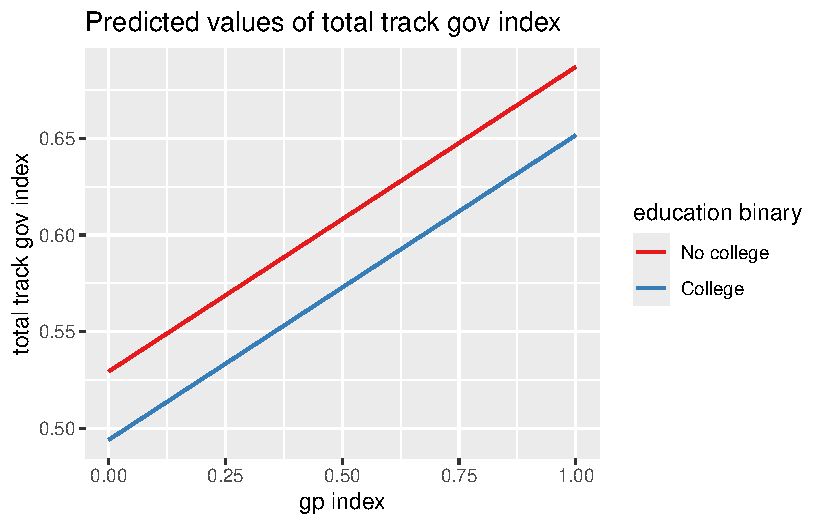
\includegraphics{Learning-to-love-big-brother-wp_files/figure-pdf/fig-marginplotperform-1.pdf}

}

\subcaption{\label{fig-marginplotperform-1}GPI x education}

\centering{

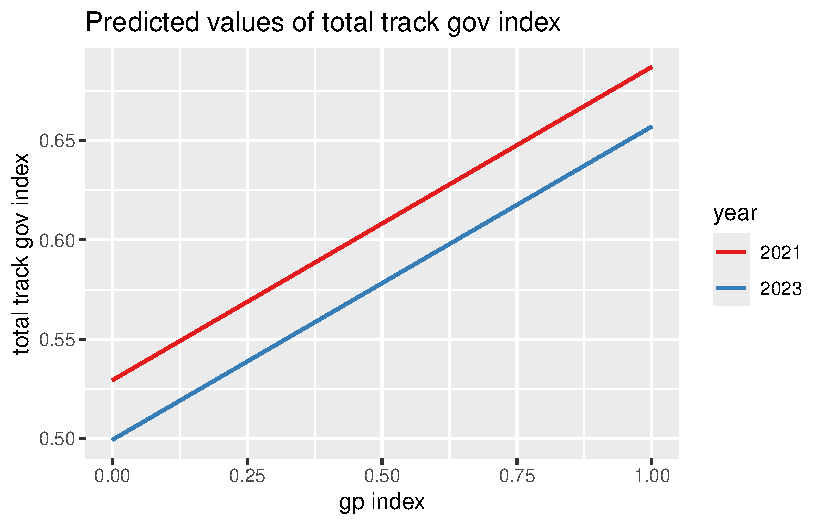
\includegraphics{Learning-to-love-big-brother-wp_files/figure-pdf/fig-marginplotperform-2.pdf}

}

\subcaption{\label{fig-marginplotperform-2}GPI x year}

}

\caption{\label{fig-marginplotperform}Marginal effect plots of
interaction terms}

\end{figure}%

As expected, government performance, controlling for demographic
factors, is a relatively strong predictor of acceptance of government
performance. According to the model, a positive view of government
performance is associated with an increased acceptance of government
monitoring. However, the relationship is likely more complex than this
story, particularly given the tumultuous events of the 2022 Covid-19
lockdowns in China. To further explore how these factors interact with
each other, the next section develops a mediation model to better
understand how this relationship may have changed due to the events of
2022.

\subsection{Changing attitudes since the
pandemic}\label{changing-attitudes-since-the-pandemic}

The following directed acyclic graph (DAG) indicates the hypothesized
causal process that generates the observed outcome variable, tracking
acceptance. In Figure~\ref{fig-dag}, \texttt{TA} represents tracking
acceptance, \texttt{GP} represents government performance approval,
\texttt{DEMO} represents demographic characteristics, and \texttt{COVID}
represents respondents' Covid-19 experience.

\begin{figure}

\centering{

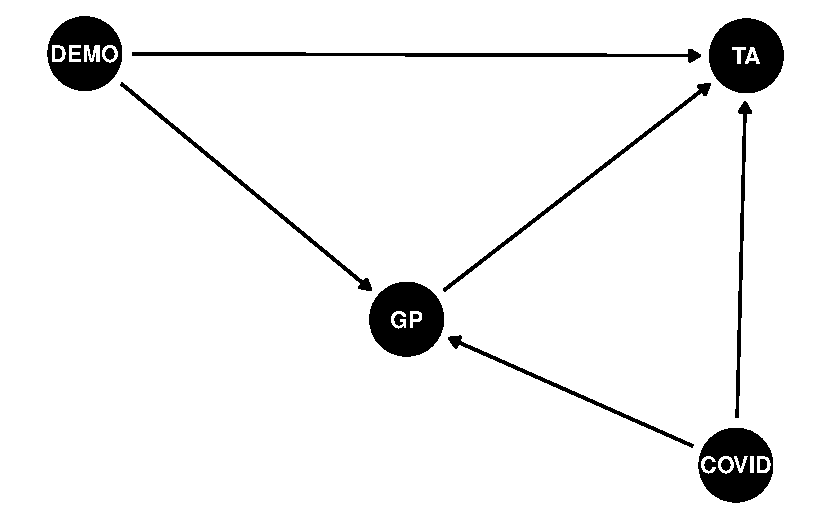
\includegraphics{Learning-to-love-big-brother-wp_files/figure-pdf/fig-dag-1.pdf}

}

\caption{\label{fig-dag}Causal process}

\end{figure}%

To operationalize this model, the first step is to create a latent
demographics construct with the demographic variables previously used in
regressions in the earlier sections loading onto this construct.
\texttt{COVID} is operationalized by the \texttt{year} variable.
Admittedly, this is not a precise mapping. The \texttt{year} variable
actually measures all changes between survey waves not accounted for by
other variables. With respect to government tracking acceptance
attitudes, however, this assumption can be justified by the fact that
the Covid-19 experience was both a daily and often traumatic one for the
Chinese public; it was a time period that involved constant and invasive
technological monitoring. If the model does indicate that the
\texttt{year} variable predicts significant change in the response
variable over the two year difference between survey waves, it would be
hard to imagine any other plausible cause. Nevertheless, it is important
to keep in mind that it is only a proxy measurement. These variables
(\texttt{year} for \texttt{COVID}, \texttt{GP}, \texttt{TA}, and
\texttt{DEMO}) are entered into a structural equation model with paths
constrained to that described by the DAG in Figure~\ref{fig-dag} and
then the parameters are estimated using the \texttt{lavaan} library in
\texttt{R}.

\begin{table}

\caption{\label{tbl-mediationmodel}Mediation model results}

\centering{

\centering
\begin{tabular}[t]{lc}
\toprule
  & (1)\\
\midrule
DEMO to GP & \num{-0.008}\\
 & \vphantom{1} (\num{0.005})\\
GP to TA & \num{0.430}***\\
 & (\num{0.015})\\
DEMO to TA & \num{-0.010}*\\
 & (\num{0.005})\\
COVID to TA & \num{0.053}***\\
 & (\num{0.006})\\
COVID to GP & \num{-0.037}***\\
 & (\num{0.007})\\
DEMO to GP to TA & \num{-0.003}\\
 & (\num{0.002})\\
COVID to GP to TA & \num{-0.002}***\\
 & (\num{0.000})\\
\midrule
Num.Obs. & \num{3507}\\
AIC & \num{52129.6}\\
BIC & \num{52246.7}\\
\bottomrule
\multicolumn{2}{l}{\rule{0pt}{1em}+ p $<$ 0.1, * p $<$ 0.05, ** p $<$ 0.01, *** p $<$ 0.001}\\
\multicolumn{2}{l}{\rule{0pt}{1em}Demographic factor variable loadings omitted}\\
\end{tabular}

}

\end{table}%

The results from this analysis in Table~\ref{tbl-mediationmodel} confirm
some of the previous findings and also reveal some interesting new
features of the data. As before, government performance plays an
important role in determining tracking acceptance. Similarly,
demographic questions do help predict tracking acceptance, but only by a
little bit. Demographics do not help predict views on government
performance, and therefore, it is not surprising that demographics does
not have an indirect effect on tracking acceptance through government
performance either. However, the Covid-19 experience, as operationalized
by the year variable, does 1) positively increase tracking acceptance
(direct path) 2) negatively decreases government performance evaluations
(direct path) and 3) negatively decreases tracking acceptance through
government performance evaluations (indirect path). The size of the
coefficients indicates that the sum of the effects is still positive on
tracking acceptance. These results indicate that the Covid-19 experience
in China did have the effect identified by You et al. (2024), which did
result in the hypothesized decrease in acceptance of government
tracking. However, this decrease in support was cancelled out by the
direct effect of Covid-19 on acceptance of tracking. However, this
decrease in support was cancelled out by the direct effect of Covid-19
on acceptance of tracking. A plausible interpretation of this is that,
as Kostka and Habich-Sobiegalla (2024) has found, respondents agree that
the tracking during Covid-19 lockdowns was necessary, but, because of
the government incompetence in responding to the spread of the virus,
they were a little less likely to positively agree than they might
otherwise have been.

\subsection{Comparing attitudes to private
monitoring}\label{comparing-attitudes-to-private-monitoring}

Finally, it is interesting to compare the determinants of government
tracking attitudes with those that determine attitudes toward private
tracking of personal information. T compare these two,
Table~\ref{tbl-privatepublic} includes models that use the previous
acceptance of government tracking index (\texttt{Public\ TA}) as the
variable alongside a similarly constructed index variable that measures
acceptance of private monitoring (\texttt{Private\ TA}).

\begin{table}

\caption{\label{tbl-privatepublic}Comparison of public vs.~private
tracking acceptance}

\centering{

\centering
\begin{tabular}[t]{lcccccc}
\toprule
\multicolumn{1}{c}{ } & \multicolumn{3}{c}{Public TA} & \multicolumn{3}{c}{Private TA} \\
\cmidrule(l{3pt}r{3pt}){2-4} \cmidrule(l{3pt}r{3pt}){5-7}
  & (1a) & (1b) & (1c) & (2a) & (2b) & (2c)\\
\midrule
(Intercept) & \num{0.488}*** & \num{0.576}*** & \num{0.214}*** & \num{0.270}*** & \num{0.432}*** & \num{0.344}***\\
 & (\num{0.021}) & (\num{0.022}) & (\num{0.021}) & (\num{0.025}) & (\num{0.026}) & (\num{0.027})\\
Age & \num{0.002}*** & \num{0.001}*** & \num{0.001}** & \num{0.000} & \num{-0.001}** & \num{-0.001}**\\
 & (\num{0.000}) & (\num{0.000}) & (\num{0.000}) & (\num{0.000}) & (\num{0.000}) & (\num{0.000})\\
College education & \num{0.006} & \num{0.014}+ & \num{0.012}+ & \num{-0.027}** & \num{-0.010} & \num{-0.010}\\
 & (\num{0.008}) & (\num{0.008}) & (\num{0.007}) & (\num{0.009}) & (\num{0.009}) & \vphantom{1} (\num{0.009})\\
Middle income & \num{-0.003} & \num{0.001} & \num{-0.003} & \num{-0.059}*** & \num{-0.049}*** & \num{-0.049}***\\
 & (\num{0.008}) & (\num{0.008}) & (\num{0.007}) & (\num{0.009}) & (\num{0.009}) & (\num{0.009})\\
High income & \num{-0.024} & \num{-0.014} & \num{-0.013} & \num{-0.027} & \num{-0.004} & \num{-0.002}\\
 & (\num{0.017}) & (\num{0.017}) & (\num{0.015}) & (\num{0.019}) & (\num{0.020}) & (\num{0.020})\\
Male & \num{-0.009} & \num{-0.004} & \num{-0.005} & \num{-0.006} & \num{0.006} & \num{0.007}\\
 & (\num{0.007}) & (\num{0.007}) & (\num{0.006}) & (\num{0.008}) & (\num{0.008}) & \vphantom{1} (\num{0.008})\\
Not a party member & \num{-0.030}** & \num{-0.032}** & \num{-0.028}** & \num{-0.010} & \num{-0.016} & \num{-0.017}\\
 & (\num{0.010}) & (\num{0.010}) & (\num{0.009}) & (\num{0.012}) & (\num{0.012}) & (\num{0.012})\\
Location: small city & \num{-0.003} & \num{0.002} & \num{-0.006} & \num{-0.043}** & \num{-0.032}* & \num{-0.033}*\\
 & (\num{0.011}) & (\num{0.011}) & (\num{0.010}) & (\num{0.013}) & (\num{0.013}) & (\num{0.013})\\
Location: mid city & \num{0.000} & \num{0.008} & \num{-0.001} & \num{-0.056}*** & \num{-0.038}** & \num{-0.039}**\\
 & (\num{0.012}) & (\num{0.012}) & (\num{0.011}) & (\num{0.014}) & (\num{0.014}) & (\num{0.014})\\
Location: big city & \num{0.001} & \num{0.013} & \num{0.011} & \num{-0.051}*** & \num{-0.024}+ & \num{-0.024}+\\
 & (\num{0.012}) & (\num{0.012}) & (\num{0.010}) & (\num{0.014}) & (\num{0.014}) & (\num{0.014})\\
Year 2023 & \num{0.039}*** & \num{0.036}*** & \num{0.052}*** & \num{0.006} & \num{0.001} & \num{0.005}\\
 & (\num{0.007}) & (\num{0.007}) & (\num{0.006}) & (\num{0.008}) & (\num{0.008}) & (\num{0.008})\\
TSI & \num{0.118}*** &  &  & \num{0.252}*** &  & \\
 & (\num{0.017}) &  &  & (\num{0.021}) &  & \\
KI &  & \num{-0.058}** &  &  & \num{-0.069}** & \\
 &  & (\num{0.022}) &  &  & (\num{0.027}) & \\
GPI &  &  & \num{0.431}*** &  &  & \num{0.071}***\\
 &  &  & (\num{0.015}) &  &  & (\num{0.020})\\
\midrule
Num.Obs. & \num{3507} & \num{3507} & \num{3507} & \num{3507} & \num{3507} & \num{3507}\\
R2 & \num{0.029} & \num{0.018} & \num{0.207} & \num{0.057} & \num{0.018} & \num{0.020}\\
F & \num{9.539} & \num{5.928} & \num{82.827} & \num{19.081} & \num{5.865} & \num{6.450}\\
\bottomrule
\multicolumn{7}{l}{\rule{0pt}{1em}+ p $<$ 0.1, * p $<$ 0.05, ** p $<$ 0.01, *** p $<$ 0.001}\\
\multicolumn{7}{l}{\rule{0pt}{1em}Reference values: no college education, low income, female, party member, countryside}\\
\multicolumn{7}{l}{\rule{0pt}{1em}Standard deviation of Public TA is:  0.2}\\
\multicolumn{7}{l}{\rule{0pt}{1em}Standard deviation of Private TA is:  0.24}\\
\end{tabular}

}

\end{table}%

The results here suggest that the determinants of attitudes towards
private company tracking are somewhat different than those that
determine attitudes towards public tracking. The \texttt{year} variable
is not significant for the private tracking models, while the tech savvy
coefficient has roughly doubled. Unsurprisingly, government performance
is also not related to private tracking acceptance. Finally, the
intercept is generally lower for private tracking acceptance, indicating
that respondents are less willing to accept private tracking, all things
being equal.

These results lend support to the hypothesis that acceptance of public
tracking has different determinants than those for private tracking and
also supports previous research that finds a significant difference
between acceptance of these two types of monitoring. The \texttt{year}
variable being insignificant for the private tracking indicates that the
pandemic-era tracking was not perceived as being fundamentally related
to commercial monitoring.

\section{Conclusion}\label{sec-conclusion}

\newpage{}

\section{References}\label{references}

\phantomsection\label{refs}
\begin{CSLReferences}{1}{1}
\bibitem[\citeproctext]{ref-abramova2022}
Abramova O, Wagner A, Olt CM, et al. (2022)
\href{https://doi.org/10.1016/j.ijinfomgt.2022.102473}{One for all, all
for one: Social considerations in user acceptance of contact tracing
apps using longitudinal evidence from germany and switzerland}.
\emph{International Journal of Information Management} 64: 102473.

\bibitem[\citeproctext]{ref-anwar2017}
Anwar M, He W, Ash I, et al. (2017)
\href{https://doi.org/10.1016/j.chb.2016.12.040}{Gender difference and
employees' cybersecurity behaviors}. \emph{Computers in Human Behavior}
69: 437--443.

\bibitem[\citeproctext]{ref-wuhanlo2021}
\emph{BBC News} (2021)
\href{https://www.bbc.com/news/world-asia-china-55628488}{Wuhan
lockdown: A year of china's fight against the covid pandemic}. Epub
ahead of print 22 January 2021.

\bibitem[\citeproctext]{ref-buxfcchi2021}
Büchi M, Festic N, Just N, et al. (2021) Digital inequalities in online
privacy protection: Effects of age, education and gender. Edward Elgar
Publishing, p. 296310.

\bibitem[\citeproctext]{ref-chen2017}
Chen D (2017) \href{https://doi.org/10.1177/1065912917691360}{Local
Distrust and Regime Support: Sources and Effects of Political Trust in
China}. \emph{Political Research Quarterly} 70(2): 314--326.

\bibitem[\citeproctext]{ref-dupree2016}
Dupree JL, Devries R, Berry DM, et al. (2016) Privacy personas:
Clustering users via attitudes and behaviors toward security practices.
In: New York, NY, USA, 7 May 2016, p. 52285239. CHI '16. Association for
Computing Machinery. Available at:
\url{https://dl.acm.org/doi/10.1145/2858036.2858214}.

\bibitem[\citeproctext]{ref-garrett2021}
Garrett PM, White JP, Lewandowsky S, et al. (2021)
\href{https://doi.org/10.1371/journal.pone.0244827}{The acceptability
and uptake of smartphone tracking for COVID-19 in Australia}. \emph{PLOS
ONE} 16(1): e0244827.

\bibitem[\citeproctext]{ref-gerber2012}
Gerber AS and Green DP (2012) \emph{Field Experiments: Design, Analysis,
and Interpretation}. New York: WW Norton.

\bibitem[\citeproctext]{ref-glynn2013}
Glynn AN (2013) \href{https://doi.org/10.1093/poq/nfs070}{What can we
learn with statistical truth serum?design and analysis of the list
experiment}. \emph{Public Opinion Quarterly} 77(S1): 159--172.

\bibitem[\citeproctext]{ref-habich-sobiegalla2023}
Habich-Sobiegalla S and Kostka G (2023)
\href{https://doi.org/10.1080/1369118X.2022.2113421}{Sharing is caring:
Willingness to share personal data through contact tracing apps in
china, germany, and the US}. \emph{Information, Communication \&
Society} 26(14): 2797--2824.

\bibitem[\citeproctext]{ref-ioannou2021}
Ioannou A and Tussyadiah I (2021)
\href{https://doi.org/10.1016/j.techsoc.2021.101774}{Privacy and
surveillance attitudes during health crises: Acceptance of surveillance
and privacy protection behaviours}. \emph{Technology in Society} 67:
101774.

\bibitem[\citeproctext]{ref-kostka2023}
Kostka G (2023) \href{https://doi.org/10.1017/dap.2023.25}{Digital
doubters in different political and cultural contexts: Comparing citizen
attitudes across three major digital technologies}. \emph{Data \&
Policy} 5: e27.

\bibitem[\citeproctext]{ref-kostka2024}
Kostka G and Habich-Sobiegalla S (2024)
\href{https://doi.org/10.1177/14614448221083285}{In times of crisis:
Public perceptions toward COVID-19 contact tracing apps in China,
Germany, and the United States}. \emph{New Media \& Society} 26(4):
2256--2294.

\bibitem[\citeproctext]{ref-kostka2021}
Kostka G, Steinacker L and Meckel M (2021)
\href{https://doi.org/10.1177/09636625211001555}{Between security and
convenience: Facial recognition technology in the eyes of citizens in
China, Germany, the United Kingdom, and the United States}. \emph{Public
Understanding of Science} 30(6): 671--690.

\bibitem[\citeproctext]{ref-lee2019}
Lee H, Wong SF, Oh J, et al. (2019)
\href{https://doi.org/10.1016/j.giq.2019.01.002}{Information privacy
concerns and demographic characteristics: Data from a korean media panel
survey}. \emph{Government Information Quarterly} 36(2): 294--303.

\bibitem[\citeproctext]{ref-liu2022}
Liu C (2022) \href{https://doi.org/10.1177/02685809221084446}{Who
supports expanding surveillance? Exploring public opinion of Chinese
social credit systems}. \emph{International Sociology} 37(3): 391--412.

\bibitem[\citeproctext]{ref-malandrino2013}
Malandrino D, Scarano V and Spinelli R (2013) 2013 international
conference on social computing. In: September 2013, pp. 57--62.
Available at:
\url{https://ieeexplore.ieee.org/abstract/document/6693312}.

\bibitem[\citeproctext]{ref-mao2022}
Mao (2022)
\href{https://www.bbc.com/news/world-asia-china-63855508}{China abandons
key parts of zero-covid strategy after protests}. \emph{BBC News}. Epub
ahead of print 7 December 2022.

\bibitem[\citeproctext]{ref-moseson2017}
Moseson H, Treleaven E, Gerdts C, et al. (2017)
\href{https://doi.org/10.1111/sifp.12042}{The List Experiment for
Measuring Abortion: What We Know and What We Need}. \emph{Studies in
Family Planning} 48(4): 397--405.

\bibitem[\citeproctext]{ref-ong}
Ong E-I and Loo WL (n.d.) Gauging the Acceptance of Contact Tracing
Technology: An Empirical Study of Singapore Residents' Concerns and
Trust in Information Sharing. DOI:
\href{https://doi.org/10.2139/ssrn.3817972}{10.2139/ssrn.3817972}.

\bibitem[\citeproctext]{ref-pavone2012}
Pavone V and Esposti SD (2012)
\href{https://doi.org/10.1177/0963662510376886}{Public assessment of new
surveillance-oriented security technologies: Beyond the trade-off
between privacy and security}. \emph{Public Understanding of Science}
21(5): 556--572.

\bibitem[\citeproctext]{ref-redlawsk2010}
Redlawsk DP, Tolbert CJ and Franko W (2010)
\href{https://doi.org/10.1177/1065912910373554}{Voters, Emotions, and
Race in 2008: Obama as the First Black President}. \emph{Political
Research Quarterly} 63(4): 875--889.

\bibitem[\citeproctext]{ref-sheehan2002}
Sheehan KB (2002)
\href{https://doi.org/10.1080/01972240252818207}{Toward a typology of
internet users and online privacy concerns}. \emph{The Information
Society} 18(1): 21--32.

\bibitem[\citeproctext]{ref-steinhardt2022}
Steinhardt HC, Holzschuh L and MacDonald AW (2022) Dreading big brother
or dreading big profit? Privacy concerns toward the state and companies
in China. \emph{First Monday}. Epub ahead of print 13 December 2022.
DOI:
\href{https://doi.org/10.5210/fm.v27i12.12679}{10.5210/fm.v27i12.12679}.

\bibitem[\citeproctext]{ref-truxfcdinger2017}
Trüdinger E-M and Steckermeier LC (2017)
\href{https://doi.org/10.1016/j.giq.2017.07.003}{Trusting and
controlling? Political trust, information and acceptance of surveillance
policies: The case of germany}. \emph{Government Information Quarterly}
34(3): 421--433.

\bibitem[\citeproctext]{ref-wnuk2020}
Wnuk A, Oleksy T and Maison D (2020)
\href{https://doi.org/10.1371/journal.pone.0238973}{The acceptance of
Covid-19 tracking technologies: The role of perceived threat, lack of
control, and ideological beliefs}. \emph{PLOS ONE} 15(9): e0238973.

\bibitem[\citeproctext]{ref-you2024}
You Y, Ma D and Chen C (2024)
\href{https://doi.org/10.1007/s11366-023-09874-y}{Public Trust During a
Public Health Crisis: Evaluating the Immediate Effects of the Pandemic
on Institutional Trust}. \emph{Journal of Chinese Political Science}
29(1): 1--29.

\bibitem[\citeproctext]{ref-zhong2014}
Zhong Y (2014) Do Chinese People Trust Their Local Government, and Why?
\emph{Problems of Post-Communism}. Epub ahead of print 1 May 2014. DOI:
\href{https://doi.org/10.2753/PPC1075-8216610303}{10.2753/PPC1075-8216610303}.

\end{CSLReferences}

\newpage{}

\section{Appendix}\label{sec-appendix}

\subsection{Index variable
definitions}\label{index-variable-definitions}

\begin{table}

\caption{\label{tbl-indexvars}Index variable component questions}

\centering{

\centering
\begin{tabular}[t]{l|l}
\hline
Q1 & How would you rate your general ability to use a computer?\\
\hline
Q2 & How would you rate your skill at fixing a computer?\\
\hline
Q3 & How would you rate your ability to program a computer?\\
\hline
\end{tabular}

\centering
\begin{tabular}[t]{l|l}
\hline
Q1 & I am very concerned about my privacy online\\
\hline
Q2 & I spend a lot of time reading about technology related privacy issues\\
\hline
Q3 & In the last year, I have had discussions with my friends about online privacy issues\\
\hline
Q4 & I feel like I know exactly how much privacy I have online\\
\hline
Q5 & Have you heard of the social credit system (official terminology)?\\
\hline
\end{tabular}

\centering
\begin{tabular}[t]{l|>{\raggedright\arraybackslash}p{5in}}
\hline
Q1 & Overall, I’m happy with the performance of the central government\\
\hline
\cellcolor{gray!6}{Q2} & \cellcolor{gray!6}{Overall, I’m happy with the performance of my local government}\\
\hline
\end{tabular}

}

\end{table}%



\end{document}
